\documentclass{article}
  \usepackage[utf8]{inputenc}
  \usepackage{graphicx}
  \usepackage{hyperref}
  \usepackage{tabulary}
  \usepackage{tabu}
  \usepackage[finnish]{babel}
  \graphicspath{{./}}
  \newcommand{\code}[1]{\texttt{#1}}
\begin{document}
\title{Tietokantasovellusharjoitustyö}
\author{Sami Kukkonen\\Helsingin yliopisto\\\texttt{sami.m.kukkonen@helsinki.fi}}
\date{\today}
\maketitle
\section{Johdanto}
Tällä kurssilla toteutan digitaalisen kuntosalilokikirjan.
Kuntosalilokikirjaan tallennetaan yksinkertaisimmillaan tehty liike, toistojen sekä suorituskokonaisuuksien (settien) määrä ja paino, jolla liike on tehty.
Järjestelmä on siis tarkoitettu tavoitteellisen painonnostoharrastuksen tukemiseen.
\par
Järjestelmä toteutetaan TypeScript\footnote{\url{http://typescriptlang.org}} (TS)-kielellä käyttäen Node.js\footnote{\url{http://nodejs.org}}-alustaa. TS-koodi käännetään JavaScriptiksi (JS), jolloin lopputulos vastaa normaalia Node.js-palvelinohjelmaa. Alkuvaiheen ideana on tutkia, onnistuuko React\footnote{\url{http://reactjs.org}}-kirjaston käyttö staattisessa palvelinympäristössä siten, että kurssilla ei tarvitse käyttää turhaa aikaa kokonaisen Single Page Architecture -selainsovelluksen rakentamiseen vaan Reactia voitaisiin käyttää staattisesti palvelinpuolella sivujen renderöintiin. Tietokantana käytetään PostgreSQL\footnote{\url{http://postgresql.org}}-relaatiotietokantaa ja koko sovellus \textit{deployataan} Herokuun\footnote{\url{http://heroku.com}}.
\section{Käyttötapaukset ja käyttäjäryhmät}
Järjestelmän käyttäjäryhmät ovat seuraavat:
\begin{description}
  \item [Vieralija] Vierailijalla tarkoitetaan henkilöä, joka käyttää järjestelmää, mutta ei ole rekisteröitynyt.
  \item [Käyttäjä] Käyttäjällä tarkoitetaan henkilöä, joka käyttää järjestelmää ja on rekisteröitynyt sekä tunnistautunut järjestelmään.
\end{description}
Vierailijan käyttötapaukset ovat seuraavat: vierailija voi
\begin{enumerate}
  \item rekisteröityä palvelun käyttäjäksi
  \item tunnistautua palvelun käyttäjäksi
\end{enumerate}
Käyttäjä voi vastaavasti:
\begin{enumerate}
  \item lisätä, muokata, poistaa sekä nähdä tallentamansa liikkeet
  \item lisätä, muokata, poistaa sekä nähdä yhden harjoituskerran, joka koostuu edellisen kohdan liikkeistä, joihin on liitetty myös toistojen määrä, settien määrä sekä paino kilogrammoissa
  \item lisätä, muokata, poistaa sekä nähdä harjoituspohjia, joiden perusteella käyttäjä voi helposti luoda uusia harjoituskertoja ilman, että käyttäjän tarvitsee lisätä jokainen setti ja toistojen määrä erikseen joka harjoituskerralla.
  \item nähdä tilastoja omista suorituksistaan
  \item muokata omia käyttäjätietojaan sekä poistaa tietonsa järjestelmästä
  \item kirjautua ulos järjestelmästä
  \item viedä omat tietonsa CSV-muodossa ulos järjestelmästä (ei vielä varmaa)
\end{enumerate}
Käyttäjäryhmien ja -tapausten suhdetta toisiinsa on havainnollistettu kuvassa \ref{fig:usecases}.
\begin{figure}
  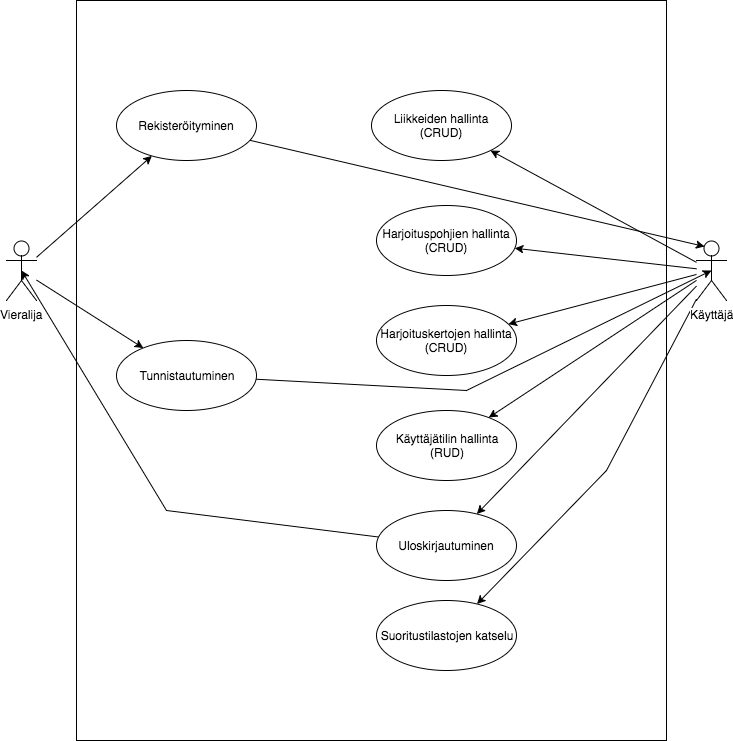
\includegraphics[width=\textwidth]{kayttotapauskaavio.png}
  \caption{Järjestelmän käyttötapauskaavio}
  \label{fig:usecases}
\end{figure}
\pagebreak
\section{Järjestelmän tietomalli}
Järjestelmän tietokohteiden väliseet suhteet on kuvattu seuraavassa käsitekaaviossa:
\begin{figure}[h]
  \centering
  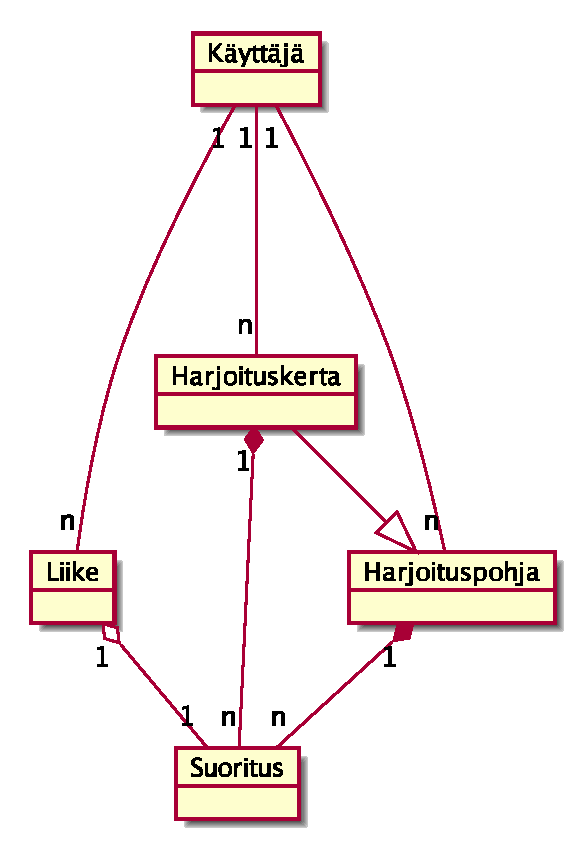
\includegraphics[width=0.5\textwidth]{tietomalli.eps}
  \caption{Käsitekaavio järjestelmän tiedosta}
\end{figure}
\\
\subsection{Tietokohteiden yksityiskohtaiset määrittelyt}
\subsubsection{Käyttäjä}
\begin{tabu} to\textwidth { | X[1,L] | X[1,L] | X[2,L] | }
  \hline
    \textbf{Attribuutti} & \textbf{Arvojoukko} & \textbf{Kuvailu} \\
  \hline
    Nimi & Merkkijono, max. 256 merkkiä & \\
  \hline
    Sähköpostiosoite & Merkkijono, max. 256 merkkiä & \\
  \hline
    Salasana & Merkkijono & \\
  \hline
\end{tabu}

\subsubsection{Harjoituskerta}
\begin{tabu} to\textwidth { | X[1,L] | X[1,L] | X[2,L] | }
  \hline
    \textbf{Attribuutti} & \textbf{Arvojoukko} & \textbf{Kuvailu} \\
  \hline
     Aloitusaika & Aika- ja päivämäärä & \\
  \hline
     Lopetusaika & Aika- ja päivämäärä & \\
  \hline
\end{tabu}

\subsubsection{Harjoituspohja}
\begin{tabu} to\textwidth { | X[1,L] | X[1,L] | X[2,L] | }
  \hline
    \textbf{Attribuutti} & \textbf{Arvojoukko} & \textbf{Kuvailu} \\
  \hline
    Nimi & Merkkijono & Harjoituspohjan uniikki (käyttäjän kontekstissa) nimi \\
  \hline
\end{tabu}

\subsubsection{Suoritus}
\begin{tabu} to\textwidth { | X[1,L] | X[1,L] | X[2,L] | }
  \hline
    \textbf{Attribuutti} & \textbf{Arvojoukko} & \textbf{Kuvailu} \\
  \hline
    Paino & Positiivinen kokonaisluku (kg) & Harjoituksessa käytetyt painot. Vapaaehtoinen kenttä. \\ 
  \hline
    Määrä & Positiivinen kokonaisluku & Toistojen määrä \\
  \hline
\end{tabu}

\subsubsection{Liike}
\begin{tabu} to\textwidth { | X[1,L] | X[1,L] | X[2,L] | }
  \hline
    \textbf{Attribuutti} & \textbf{Arvojoukko} & \textbf{Kuvailu} \\
  \hline
    Nimi & Merkkijono & \\
  \hline
\end{tabu}

\end{document}